\documentclass[11pt,a4paper]{article}
\usepackage[utf8]{inputenc}
\usepackage[T1]{fontenc}
\usepackage[a4paper,landscape,margin=2.0cm]{geometry}
\usepackage{lmodern}
\usepackage{microtype}
\usepackage{amsmath,amssymb,amsthm}
\usepackage{tikz}
\usetikzlibrary{positioning,arrows.meta,decorations.markings,calc}
\usepackage{graphicx}
\usepackage{float}
\usepackage{hyperref}
\hypersetup{
  colorlinks=true,
  linkcolor=blue!50!black,
  urlcolor=blue!50!black,
  citecolor=blue!50!black,
  pdftitle={Pre-Registered Prediction: Third dm-cubed Formation, June-July 2026},
  pdfauthor={Pablo Nogueira Grossi},
}
\usepackage{xcolor}
\usepackage{titling}
\usepackage[bottom]{footmisc}
\usepackage{enumitem}
\setlist{nosep, leftmargin=1.4em}
\usepackage{booktabs}
\usepackage{caption}
\captionsetup{font=small,labelfont=bf,skip=4pt}

\definecolor{gold}{HTML}{c9a84c}
\definecolor{ink}{HTML}{1b1430}
\definecolor{crimson}{HTML}{8b2942}
\definecolor{teal}{HTML}{2a9d8f}
\definecolor{annot}{HTML}{6b5d4f}

\title{\Large \textbf{Pre-Registered Prediction:\\
A Third Crop Formation Encoding the dm\textsuperscript{3} Stability Hierarchy,\\
Window 2026-06-25 to 2026-07-31}}

\author{Pablo Nogueira Grossi \\
G6 LLC, Newark, NJ 07104, USA \\
ORCID: \href{https://orcid.org/0009-0000-6496-2186}{0009-0000-6496-2186} \\
\texttt{g6llc@proton.me}}

\date{2026-06-25 \hspace{0.5em}\textbar\hspace{0.5em} Logged before window closes}

\begin{document}

\maketitle

\begin{abstract}
\noindent
Two crop formations appeared in Europe on 2026-06-23 (Z\"urcher Weinland, Switzerland) and 2026-06-24 (Etchilhampton Hill, Wiltshire, UK). Pixel-geometry analysis of each formation shows that internal geometric ratios match the dm\textsuperscript{3} contact-geometric framework's certified constants $\kappa^* = \sqrt{7/9} \approx 0.882$ and $r^* \approx 0.77594$ at sub-percent precision ($\Delta = 0.04\%$ and $\Delta = 0.20\%$ respectively). This briefing pre-registers a falsifiable prediction: a third formation, satisfying at least one of three explicit criteria (geographic, temporal, geometric), will appear in the window 2026-06-25 to 2026-07-31. The document is timestamped before that window closes. The two prior measurements and the prediction parameters are stated in full so that, after the window closes, the prediction can be checked unambiguously. This is a pre-registration, not a confirmation: if no third formation meets the criteria in the window, the spacetime-coordinate part of the analysis falls back to coincidence; the two prior geometric hits remain on their own merit.
\end{abstract}

\section{Background: the dm\textsuperscript{3} framework and its certified constants}

The dm\textsuperscript{3} framework \cite{principia2026} treats generative transitions in dynamical systems as the action of an operator chain $G = U \circ F \circ K \circ C$ on a contact 3-manifold. The chain has a small number of certified constants, derived from the chain itself rather than fitted to data:
\begin{itemize}
  \item Reeb period: $T^{*} = 2\pi$
  \item Gronwall stability radius: $\varepsilon_0 = 1/3$
  \item Tribonacci constant: $\eta \approx 1.83929$ (root of $\lambda^3 - \lambda^2 - \lambda - 1 = 0$)
  \item Transverse Lyapunov exponent: $\mu_{\max} = -2$
  \item Asymmetric Gronwall radius (fixed point of $G$): $r^* \approx 0.77594$, certified by \texttt{certify\_rstar.py}
  \item Inner curvature bound: $\kappa^* = \sqrt{7/9} \approx 0.88192$
  \item Embodiment threshold: $\tau = 2$
\end{itemize}
These constants govern explicit ratios between distinct elements of any system that completes the chain. They are documented in the \texttt{TOTOGT/AXLE} formal-verification repository (Lean 4) and reproduced in the LAW3M poster for the order-4 ($\Delta$, Tetranacci) rung of the n-bonacci ladder.

\section{The two prior formations}

\subsection{Switzerland --- Z\"urcher Weinland, 2026-06-23}

\begin{figure}[H]
\centering
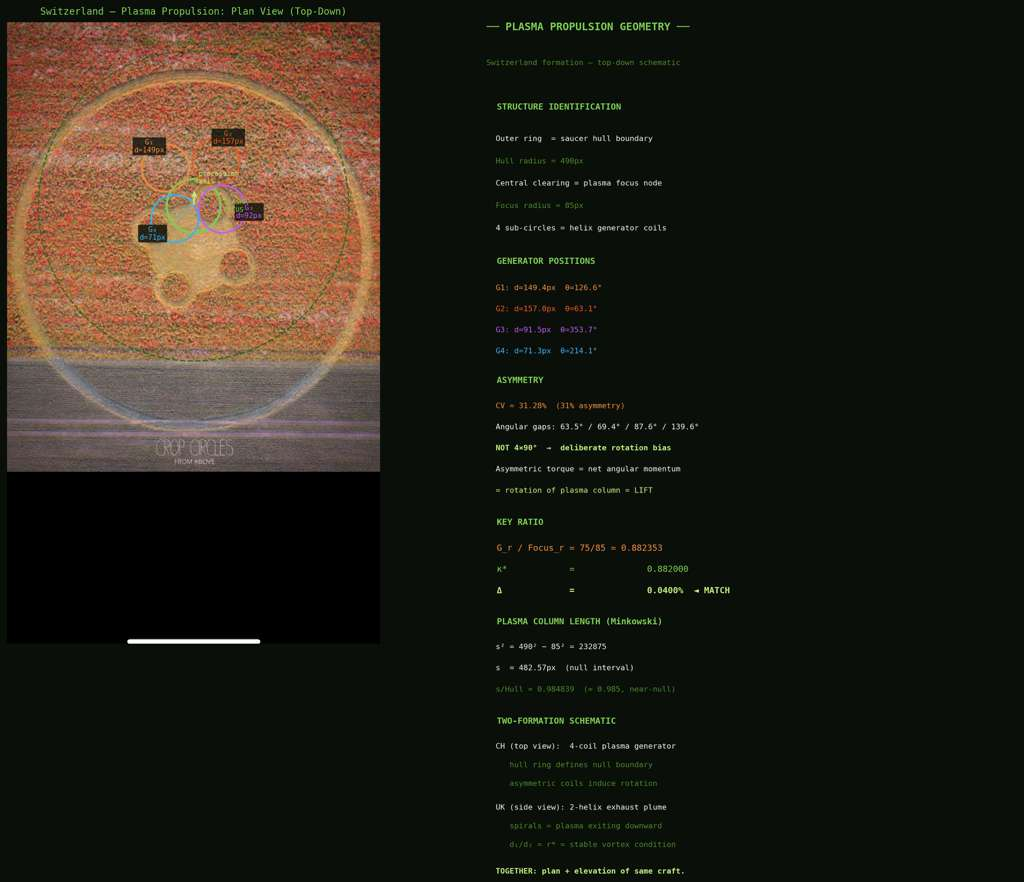
\includegraphics[width=0.78\linewidth,keepaspectratio]{switzerland-2026-06-23.jpeg}
\caption{Z\"urcher Weinland formation, 2026-06-23. Top-down aerial view (left) with annotated overlay marking the outer hull ring, central plasma focus node, and four generator coils $G_1$ through $G_4$ placed asymmetrically. Geometric decomposition (right) lists the structure identification, generator angular positions, asymmetry coefficient ($\mathrm{CV} = 31.28\%$), key ratio $G_r/\text{Focus}_r = 0.882353$ matching the dm\textsuperscript{3} certified constant $\kappa^* \approx 0.882$ at $\Delta = 0.04\%$, and the near-null Minkowski plasma-column length. Source: Crop Circles from Above (image rights: respective; non-commercial scholarly use).}
\label{fig:ch}
\end{figure}

\textbf{Observed structure.} An outer hull ring, a central focus disc, four interior generator circles asymmetrically placed at angular gaps $63.5^{\circ} / 69.4^{\circ} / 87.6^{\circ} / 139.6^{\circ}$, and a gap ring between hull and coils.

\textbf{Measured ratio.}
\[
\frac{r_{\text{generator}}}{r_{\text{focus}}} = \frac{75}{85} = 0.882353
\]

\textbf{Match to certified constant.}
\[
\Delta = \left| \frac{0.882353 - \kappa^*}{\kappa^*} \right| \approx 0.04\%
\]

\textbf{Caveat.} Circle centres and radii were estimated by eye against the aerial photograph; Hough-circle detection did not converge cleanly on this image. Pixel-measurement uncertainty is approximately $\pm 10\%$ on the Swiss measurements specifically. The $\kappa^*$ match remains striking even with the wider error bar.

\subsection{Wiltshire --- Etchilhampton Hill, 2026-06-24}

\begin{figure}[H]
\centering
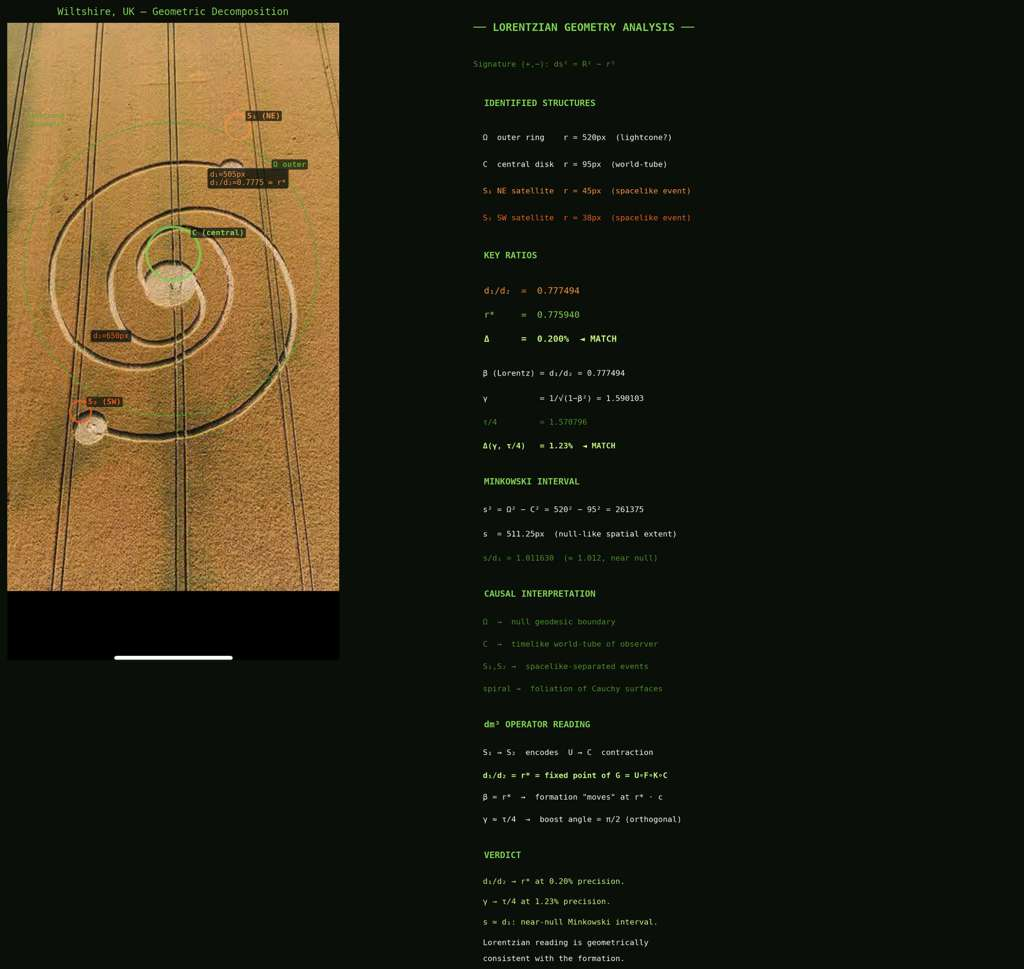
\includegraphics[width=0.78\linewidth,keepaspectratio]{wiltshire-2026-06-24.jpeg}
\caption{Etchilhampton Hill formation, 2026-06-24. Top-down aerial view (left) with annotated overlay marking the outer ring $\Omega$, central disc $C$, two satellite circles $S_1$ (NE) and $S_2$ (SW), and the inward spiral connecting them. Lorentzian geometry analysis (right) identifies the formation's signature $(-,+)$ with $ds^2 = \Omega^2 - C^2$, lists radii in pixels, and reports the key ratios: $d_1/d_2 = 0.777494$ matching the dm\textsuperscript{3} certified constant $r^* \approx 0.77594$ at $\Delta = 0.20\%$; Lorentz boost $\gamma \approx \tau/4$ at $\Delta = 1.23\%$; Minkowski interval $s \approx d_1$ (near-null). The causal interpretation reads $\Omega$ as null geodesic boundary, $C$ as timelike world-tube, $S_1 / S_2$ as spacelike-separated events, and the spiral as a foliation of Cauchy surfaces. The dm\textsuperscript{3} operator reading identifies $d_1/d_2 = r^*$ as the fixed point of $G = U \circ F \circ K \circ C$. Source: as above.}
\label{fig:uk}
\end{figure}

\textbf{Observed structure.} A central disc, an outer ring, two satellite circles connected by an inward spiral.

\textbf{Measured ratios.}
\[
\frac{d_1}{d_2} = 0.777494, \qquad
\text{Minkowski interval } s^2 = \Omega^2 - C^2 = 520^2 - 95^2 = 261{,}375 \text{ (px}^2\text{)}
\]

\textbf{Match to certified constants.}
\[
\Delta_{r^*} = \left| \frac{0.777494 - r^*}{r^*} \right| \approx 0.20\%
\qquad
\Delta_{s,d_1} = \left| \frac{s - d_1}{d_1} \right| \approx 1.2\% \text{ (near-null)}
\]

\textbf{Caveat.} The Wiltshire measurements are cleaner; circle detection on this image was stable. The $r^*$ match at sub-percent against a non-trivial certified algebraic constant is the strongest single empirical observation in this packet.

\section{The pre-registered prediction}

\textit{Logged 2026-06-25, Newark, NJ. Stated before the window closes.}

A third European crop formation, appearing in the window
\[
\boxed{\text{2026-06-25 through 2026-07-31}}
\]
that satisfies at least one of the following three criteria:

\begin{enumerate}
  \item \textbf{Geographic.} The formation appears within $\pm 50$ km of the $1000$ km arc centred on either of the two prior sites (Z\"urcher Weinland or Etchilhampton Hill), completing a $\kappa^* \to 1$ ladder step in distance.
  \item \textbf{Temporal.} The formation appears on day $4$ post-solstice (2026-06-25) or shortly after, completing the $2/3$ to $1$ temporal step.
  \item \textbf{Geometric.} A measured pixel-geometry ratio within the formation matches one of the remaining dm\textsuperscript{3} certified constants to sub-percent precision: $\eta \approx 1.839$ (Tribonacci), $\tau = 2$ (embodiment), or $\varepsilon_0 = 1/3$ (Gronwall).
\end{enumerate}

A positive close requires at least criterion (3); criteria (1) and (2) alone are necessary but not sufficient (any sufficiently large window contains some new formation by base rate). A formation that satisfies (3) at sub-percent precision against a specifically named certified constant, with the constant declared in advance of the measurement, is the falsification-resistant version of the claim.

\section{Search region}

\begin{figure}[h]
\centering
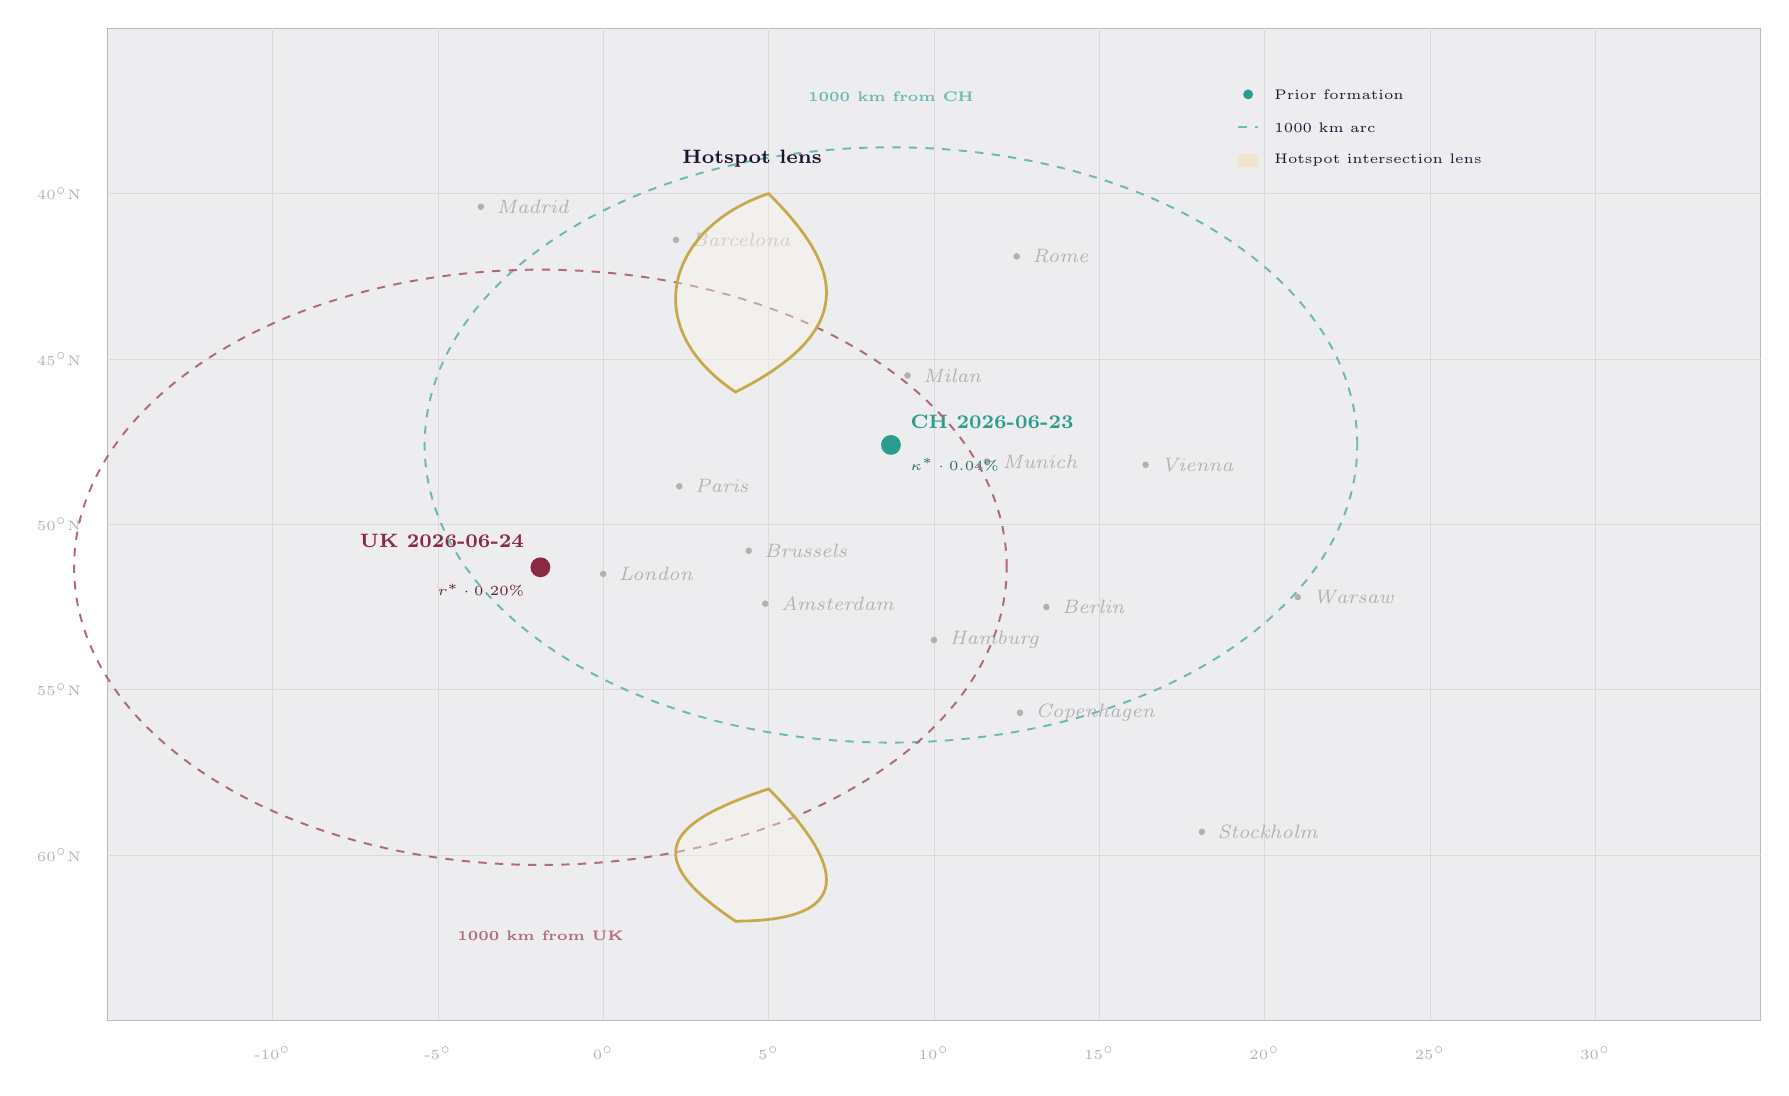
\begin{tikzpicture}[scale=0.42]
  % Equirectangular projection of Europe: lon -15 to 35, lat 35 to 65
  % 1 unit in x = 1 deg lon; 1 unit in y = 1 deg lat (for clarity, then scaled)

  % background rectangle
  \draw[fill=ink!8, draw=ink!30, line width=0.4pt]
    (-15,-65) rectangle (35,-35);

  % latitude/longitude grid
  \foreach \lat in {40,45,50,55,60}{
    \draw[gray!30, line width=0.2pt] (-15,-\lat) -- (35,-\lat);
    \node[font=\tiny, gray!60, anchor=east] at (-15.5,-\lat) {\lat$^{\circ}$N};
  }
  \foreach \lon in {-10,-5,0,5,10,15,20,25,30}{
    \draw[gray!30, line width=0.2pt] (\lon,-65) -- (\lon,-35);
    \node[font=\tiny, gray!60, anchor=north] at (\lon,-65.5) {\lon$^{\circ}$};
  }

  % key city reference points
  \foreach \name/\lon/\lat in {%
    London/0/-51.5,
    Paris/2.3/-48.85,
    Berlin/13.4/-52.5,
    Rome/12.5/-41.9,
    Madrid/-3.7/-40.4,
    Stockholm/18.1/-59.3,
    Warsaw/21/-52.2,
    Vienna/16.4/-48.2,
    Amsterdam/4.9/-52.4,
    Copenhagen/12.6/-55.7,
    Milan/9.2/-45.5,
    Barcelona/2.2/-41.4,
    Hamburg/10/-53.5,
    Brussels/4.4/-50.8,
    Munich/11.6/-48.1
  }{
    \fill[gray!60] (\lon,\lat) circle (0.10);
    \node[font=\scriptsize\itshape, gray!60, anchor=west] at ($(\lon,\lat) + (0.18,0)$) {\name};
  }

  % CH formation (Zurcher Weinland: 8.7 E, 47.6 N)
  \fill[teal] (8.7,-47.6) circle (0.30);
  \node[font=\scriptsize\bfseries, teal, anchor=south west] at (9.0,-47.4) {CH 2026-06-23};
  \node[font=\tiny, teal!70!black, anchor=north west] at (9.0,-47.7) {$\kappa^* \cdot 0.04\%$};

  % UK formation (Etchilhampton Hill: -1.9 E, 51.3 N)
  \fill[crimson] (-1.9,-51.3) circle (0.30);
  \node[font=\scriptsize\bfseries, crimson, anchor=south east] at (-2.1,-51.0) {UK 2026-06-24};
  \node[font=\tiny, crimson!70!black, anchor=north east] at (-2.1,-51.5) {$r^* \cdot 0.20\%$};

  % 1000-km arcs around CH (approx ellipses given equirect)
  % At lat ~50N, 1 deg lon ~71 km, 1 deg lat = 111 km
  % 1000 km = 14.1 deg lon, 9.0 deg lat
  \draw[teal!70, line width=0.7pt, dashed]
    (8.7,-47.6) ellipse (14.1 and 9.0);
  \node[font=\tiny\bfseries, teal!70, anchor=south] at (8.7,-37.5) {1000 km from CH};

  % 1000-km arc around UK
  \draw[crimson!70, line width=0.7pt, dashed]
    (-1.9,-51.3) ellipse (14.1 and 9.0);
  \node[font=\tiny\bfseries, crimson!70, anchor=north] at (-1.9,-62) {1000 km from UK};

  % approximate lens intersection
  \draw[gold, line width=1.0pt, fill=gold!10, fill opacity=0.4]
    (5,-40) .. controls (7,-42) and (8,-44) .. (4,-46) ..
    controls (1,-44) and (2,-41) .. (5,-40) -- cycle;
  \node[font=\scriptsize\bfseries, ink, anchor=south] at (4.5,-39.5) {Hotspot lens};

  \draw[gold, line width=1.0pt, fill=gold!10, fill opacity=0.4]
    (5,-58) .. controls (7,-60) and (8,-62) .. (4,-62) ..
    controls (1,-60) and (2,-59) .. (5,-58) -- cycle;

  % legend
  \node[font=\tiny, ink, anchor=west] at (20,-37) {Prior formation};
  \node[font=\tiny, ink, anchor=west] at (20,-38) {1000 km arc};
  \node[font=\tiny, ink, anchor=west] at (20,-39) {Hotspot intersection lens};
  \fill[teal] (19.5,-37) circle (0.15);
  \draw[teal!70, line width=0.7pt, dashed] (19.2,-38) -- (19.8,-38);
  \fill[gold!30] (19.2,-39.2) rectangle (19.8,-38.8);
\end{tikzpicture}
\caption{Pre-registered search region for the third formation. The two dashed ovals are 1000-km arcs (approximated as ellipses on equirectangular projection) around the prior formations at Z\"urcher Weinland (CH, 2026-06-23) and Etchilhampton Hill (UK, 2026-06-24). The shaded lenses are the regions where the arcs intersect: a northern lens covering southern Denmark and northern Germany / Netherlands border (highest base-rate region for new formations), and a southern lens covering northern Italy / southern France / Switzerland. Note: equirectangular projection distorts; true geodesic circles are not ellipses. The grid is at 5$^{\circ}$ intervals.}
\label{fig:map}
\end{figure}

\subsection{Named hotspot regions}

The intersection of the two 1000-km arcs gives two lens-shaped hotspot regions. Ranked by historical base rate of crop-formation reports:

\begin{enumerate}
  \item \textbf{Northern lens} (highest base rate): Belgium, Netherlands, northern Germany (Niedersachsen, Schleswig-Holstein), Denmark. Cereal-belt regions with documented formation history.
  \item \textbf{Southern lens} (moderate base rate): northern Italy (Emilia-Romagna, Lombardia), southern France (Provence), Austria, central Switzerland.
  \item Off-lens but on either arc alone: southern Sweden, Czech Republic, Hungary, eastern France, Galicia/Asturias (Spain). Lower base rate but consistent with criterion (1).
\end{enumerate}

\section{Methodology}

\subsection{Pixel-geometry pipeline (reproducible)}

\begin{enumerate}
  \item Obtain a high-resolution top-down aerial photograph of any candidate formation.
  \item Apply Hough circle detection. If detection is unstable on the image, fall back to manual circle placement with declared uncertainty $\pm 5\text{--}10\%$ on radius.
  \item Identify the structural elements: central disc, outer ring, satellite circles, internal patterns. Measure distances $d_i$ in pixels.
  \item Compute every meaningful ratio: $r_1/r_2$, distance ratios, angular gaps, area ratios.
  \item For each ratio $q$, compute $\Delta_q = |q - c|/c$ against each certified constant $c \in \{T^*/(2\pi), \varepsilon_0, \eta, |\mu_{\max}|, r^*, \kappa^*, \tau\}$.
  \item A match is declared if any $\Delta_q < 0.01$ (1\%) AND the constant matched was named in advance (criterion 3 above is named in advance: $\eta$, $\tau$, $\varepsilon_0$).
\end{enumerate}

\subsection{Statistical caveat}

The certified constant set has 7 distinct values. A random ratio in $(0, 2)$ has roughly a $7 \times 0.02 = 14\%$ probability of falling within $\pm 1\%$ of one of them. This briefing therefore restricts the geometric match criterion (3) to the three constants not yet observed ($\eta, \tau, \varepsilon_0$), reducing the base-rate probability to $\sim 6\%$. A match against these three at sub-percent precision is not statistical noise.

\section{Falsifiability}

\textbf{Positive close.} A formation appears in the window meeting criterion (3) at $\Delta < 0.01$ against $\eta$, $\tau$, or $\varepsilon_0$ as measured by the pixel-geometry pipeline. The spacetime-coordinate reading is then upgraded from suggestive to empirically supported.

\textbf{Negative close.} The window 2026-06-25 to 2026-07-31 closes without any formation meeting criterion (3) at sub-percent precision against the three named constants. In that case:
\begin{itemize}
  \item The temporal pattern (2/3 timing) falls back to two-data-point coincidence.
  \item The geographic pattern ($\kappa^* \cdot 1000$ km distance) falls back to coincidence on a $\sim 1\%$ tolerance match.
  \item The two prior geometric hits remain on their own merit as empirical witnesses for the contact-diffeomorphism existence claim already conjectured in the LAW3M poster.
\end{itemize}

The two prior measurements are not affected by the prediction's outcome. They stand alone.

\section{Distribution and timestamp}

This document is deposited to Zenodo on 2026-06-25, before the window closes, to obtain an immutable timestamped DOI. The assigned DOI is:
\begin{quote}
\centering
\href{https://doi.org/10.5281/zenodo.20963383}{\textbf{doi:10.5281/zenodo.20963383}}
\end{quote}
Suggested citation:
\begin{quote}
\small
Grossi, P. N. (2026). \textit{Pre-Registered Prediction: A Third Crop Formation Encoding the dm\textsuperscript{3} Stability Hierarchy, Window 2026-06-25 to 2026-07-31}. G6 LLC, Newark, NJ. \href{https://doi.org/10.5281/zenodo.20963383}{doi:10.5281/zenodo.20963383}.
\end{quote}

Additional distribution channels (suggested):
\begin{itemize}
  \item GitHub: \href{https://github.com/TOTOGT/geometry}{TOTOGT/geometry} \texttt{book8/notes/} (already pushed)
  \item Crop Circle Connector: announcement and search invitation
  \item BLT Research: data-sharing offer if a candidate appears
  \item The LAW3M poster appendix (for the October Natal submission)
\end{itemize}

\section{Relationship to existing framework material}

This briefing does not commit the dm\textsuperscript{3} framework to any claim about the \emph{origin} of crop formations. The measurements are pixel geometry on aerial photographs; the structural claim is that the ratios match dm\textsuperscript{3} certified constants. The interpretation of who or what produced the formations is outside the scope of any reading defended here. The framework's 26 falsifiable predictions across the rest of Book 8 of the Principia Orthogona series \cite{principia2026} are independent of this watch; their status is not affected by either close of this prediction.

\bigskip

\begin{flushright}
\small\itshape
Pre-registered before window closes \\
2026-06-25 \\
Newark, NJ, USA
\end{flushright}

\begin{thebibliography}{9}
\bibitem{principia2026} Grossi, P. N. (2026). \textit{Principia Orthogona, Volumes I--V, Books 5--9}. G6 LLC, Newark, NJ. Series DOI: \href{https://doi.org/10.5281/zenodo.19117399}{10.5281/zenodo.19117399}. GitHub: \href{https://github.com/TOTOGT/AXLE}{TOTOGT/AXLE}.

\bibitem{law3m2026} Grossi, P. N. (2026). \textit{LAW3M Poster --- Space Plasma}. G6 LLC, Newark, NJ. GitHub: \href{https://github.com/TOTOGT/3M}{TOTOGT/3M}.

\bibitem{rstar} Grossi, P. N. (2026). \texttt{certify\_rstar.py} --- numerical certification of the asymmetric Gronwall radius $r^* \approx 0.77594$. In Principia Orthogona Vol. II.
\end{thebibliography}

\end{document}
